\begin{frame}[fragile]
\frametitle{LA-CoNGA: Plataforma y Método}
\begin{columns}[c] % The "c" option specifies centered vertical alignment while the "t" option is used for top vertical alignment

\column{.60\textwidth}
\begin{itemize}\small
	\item Plataforma de {\it e-learning} integrada
	\begin{itemize}
		\item Acceso remoto a una red de laboratorios interconectados
		\item Recursos docentes
		\item Repositorios de datos e información
		\item Recursos de comunicación
		\item Computación en la nube
	\end{itemize}
	\item Currículo 
	\begin{itemize}
		\item Distribuido en bloques pequeños
		\item Orientado a la aplicación inmediata de las competencias adquiridas
	\end{itemize}
	\item Buenas prácticas
	\begin{itemize}
		\item Trabajo en colaboración científica
		\item Reproducibilidad científica
	\end{itemize}
	\item Programa de movilidad en LA y UE
	\begin{itemize}
		\item Socios Académicos y Científicos
		\item Socios Industriales
	\end{itemize}	
\end{itemize}
\column{.36\textwidth} % Right column and width
\begin{center}
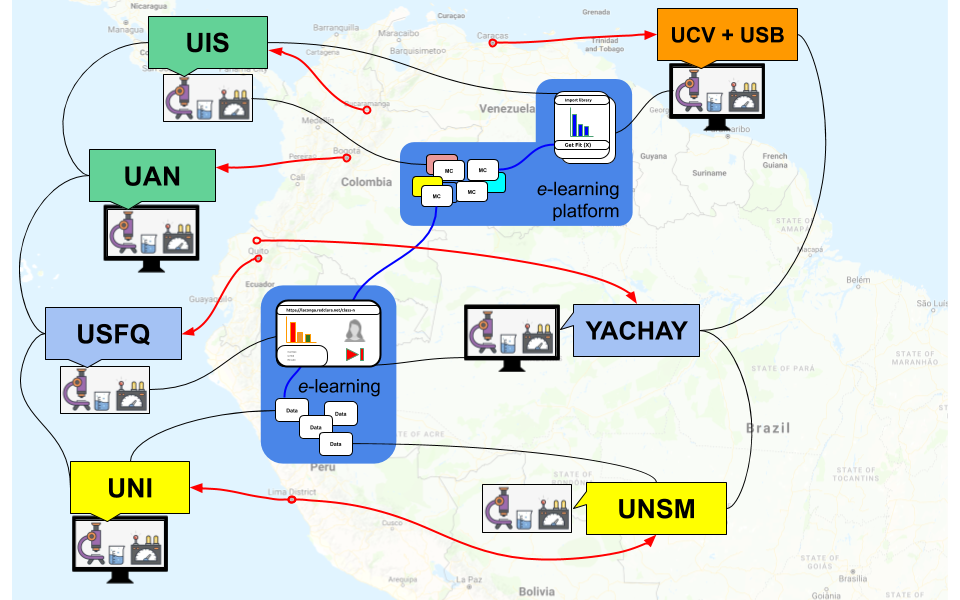
\includegraphics[scale=0.16]{imagenes/labRemotosElearning.png}
\end{center}

\begin{center}
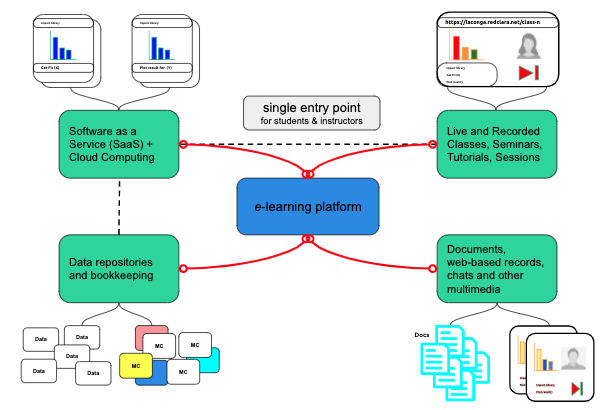
\includegraphics[scale=0.23]{imagenes/Elearning.png}
\end{center}

\end{columns}

\end{frame}

\begin{frame}[fragile]
\frametitle{LA-CoNGA: Plataforma y Método}
\begin{center}

\begin{tikzpicture}[node distance=1.25cm, auto,]
 %nodes
  \node[inner sep=0pt] (logo) at (7.2,-3)
    {
\includegraphics[scale=0.27]{imagenes/isotipo-RGB-pequeno.png}};
  \node (text) at (7.2,-3.1) {};
	\circledarrow{ultra thick, logobrown}{text}{1.7cm};
 \node[inner sep=0pt] (plataforma) at (10.4,-0.5)
    {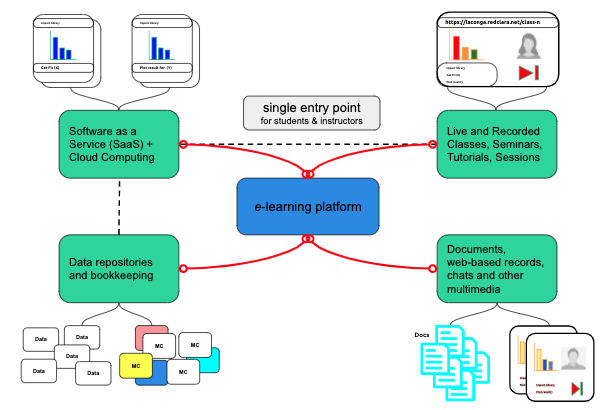
\includegraphics[scale=0.18]{imagenes/Elearning.png}};
 \node[inner sep=0pt] (tools) at (11,-3)
    {
\includegraphics[scale=0.12]{imagenes/logos/logos.png}};
 \node[inner sep=0pt] (clases) at (10,-5.7)
    {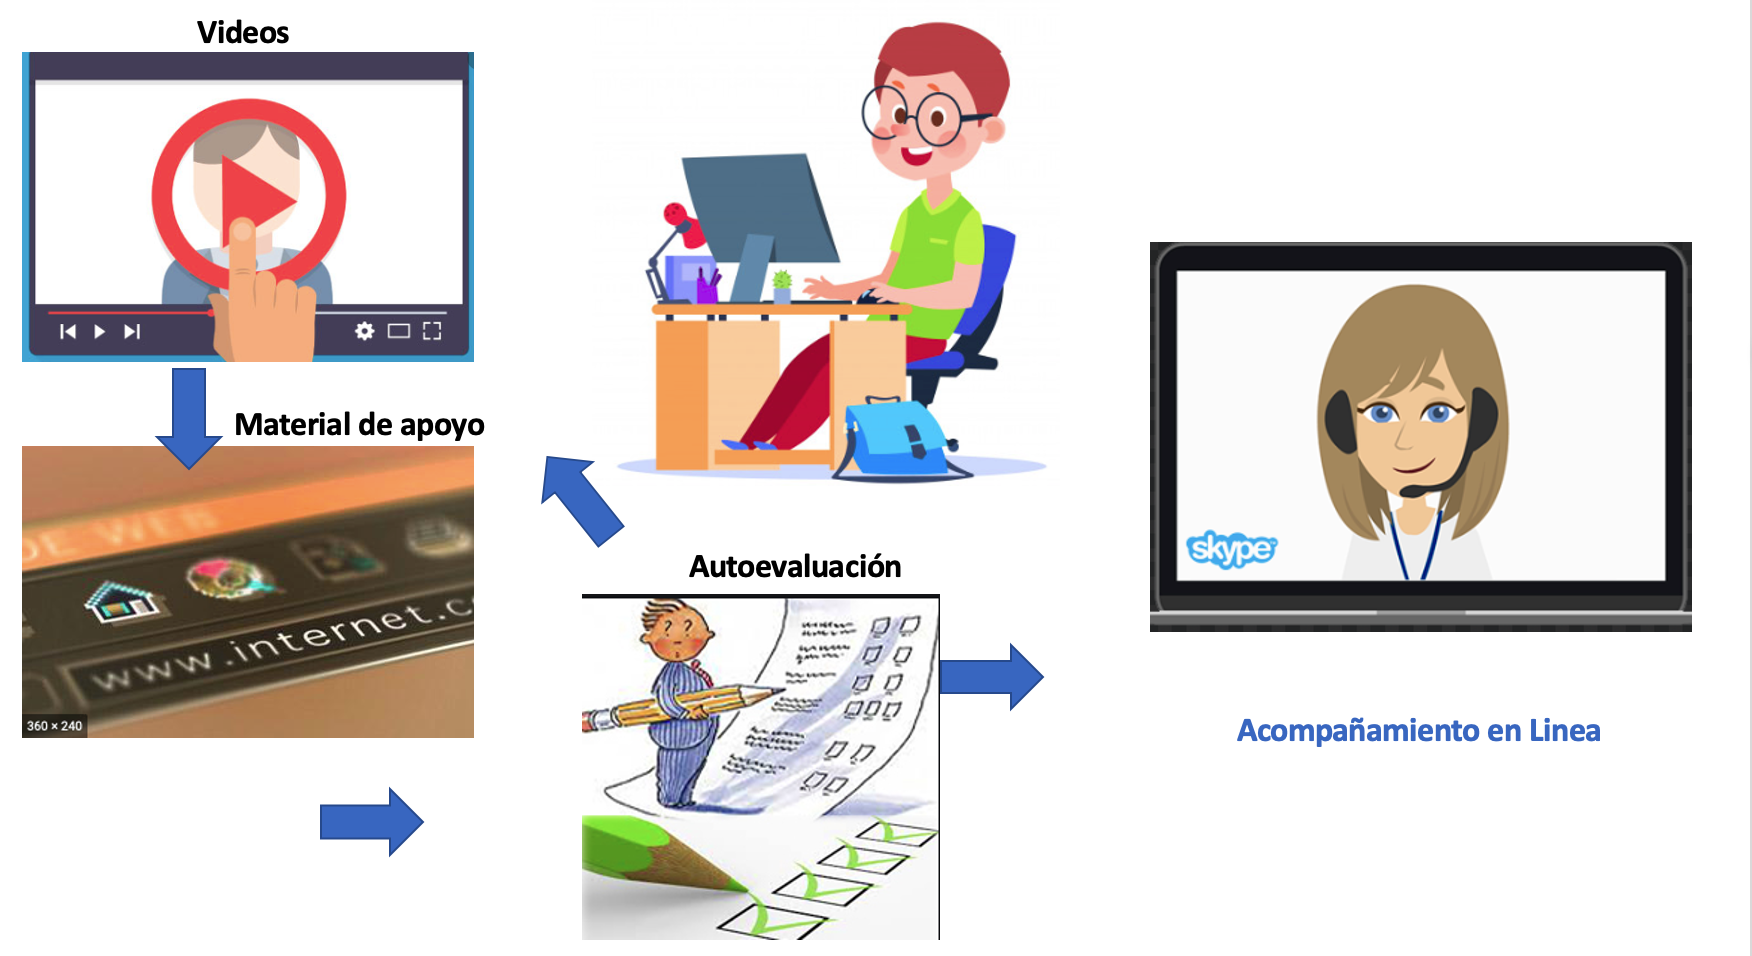
\includegraphics[scale=0.12]{imagenes/clases.png}};
 \node[inner sep=0pt] (bloques) at (5.2,-6)
    {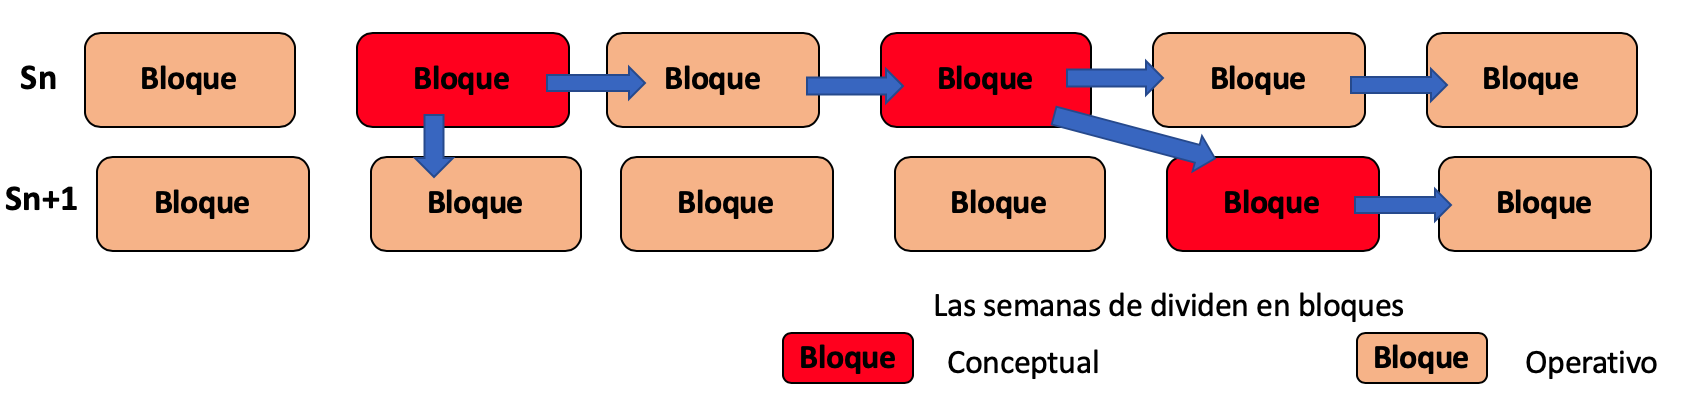
\includegraphics[scale=0.21]{imagenes/bloques.png}};
 \node[inner sep=0pt] (tools) at (3.8,-3.5)
    {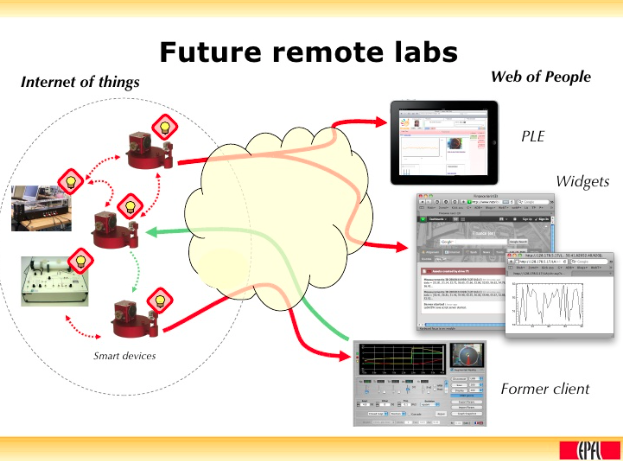
\includegraphics[scale=0.12]{imagenes/remoteLab.png}};
 \node[inner sep=0pt] (reproducibilidad) at (4.2,-0.5)
    {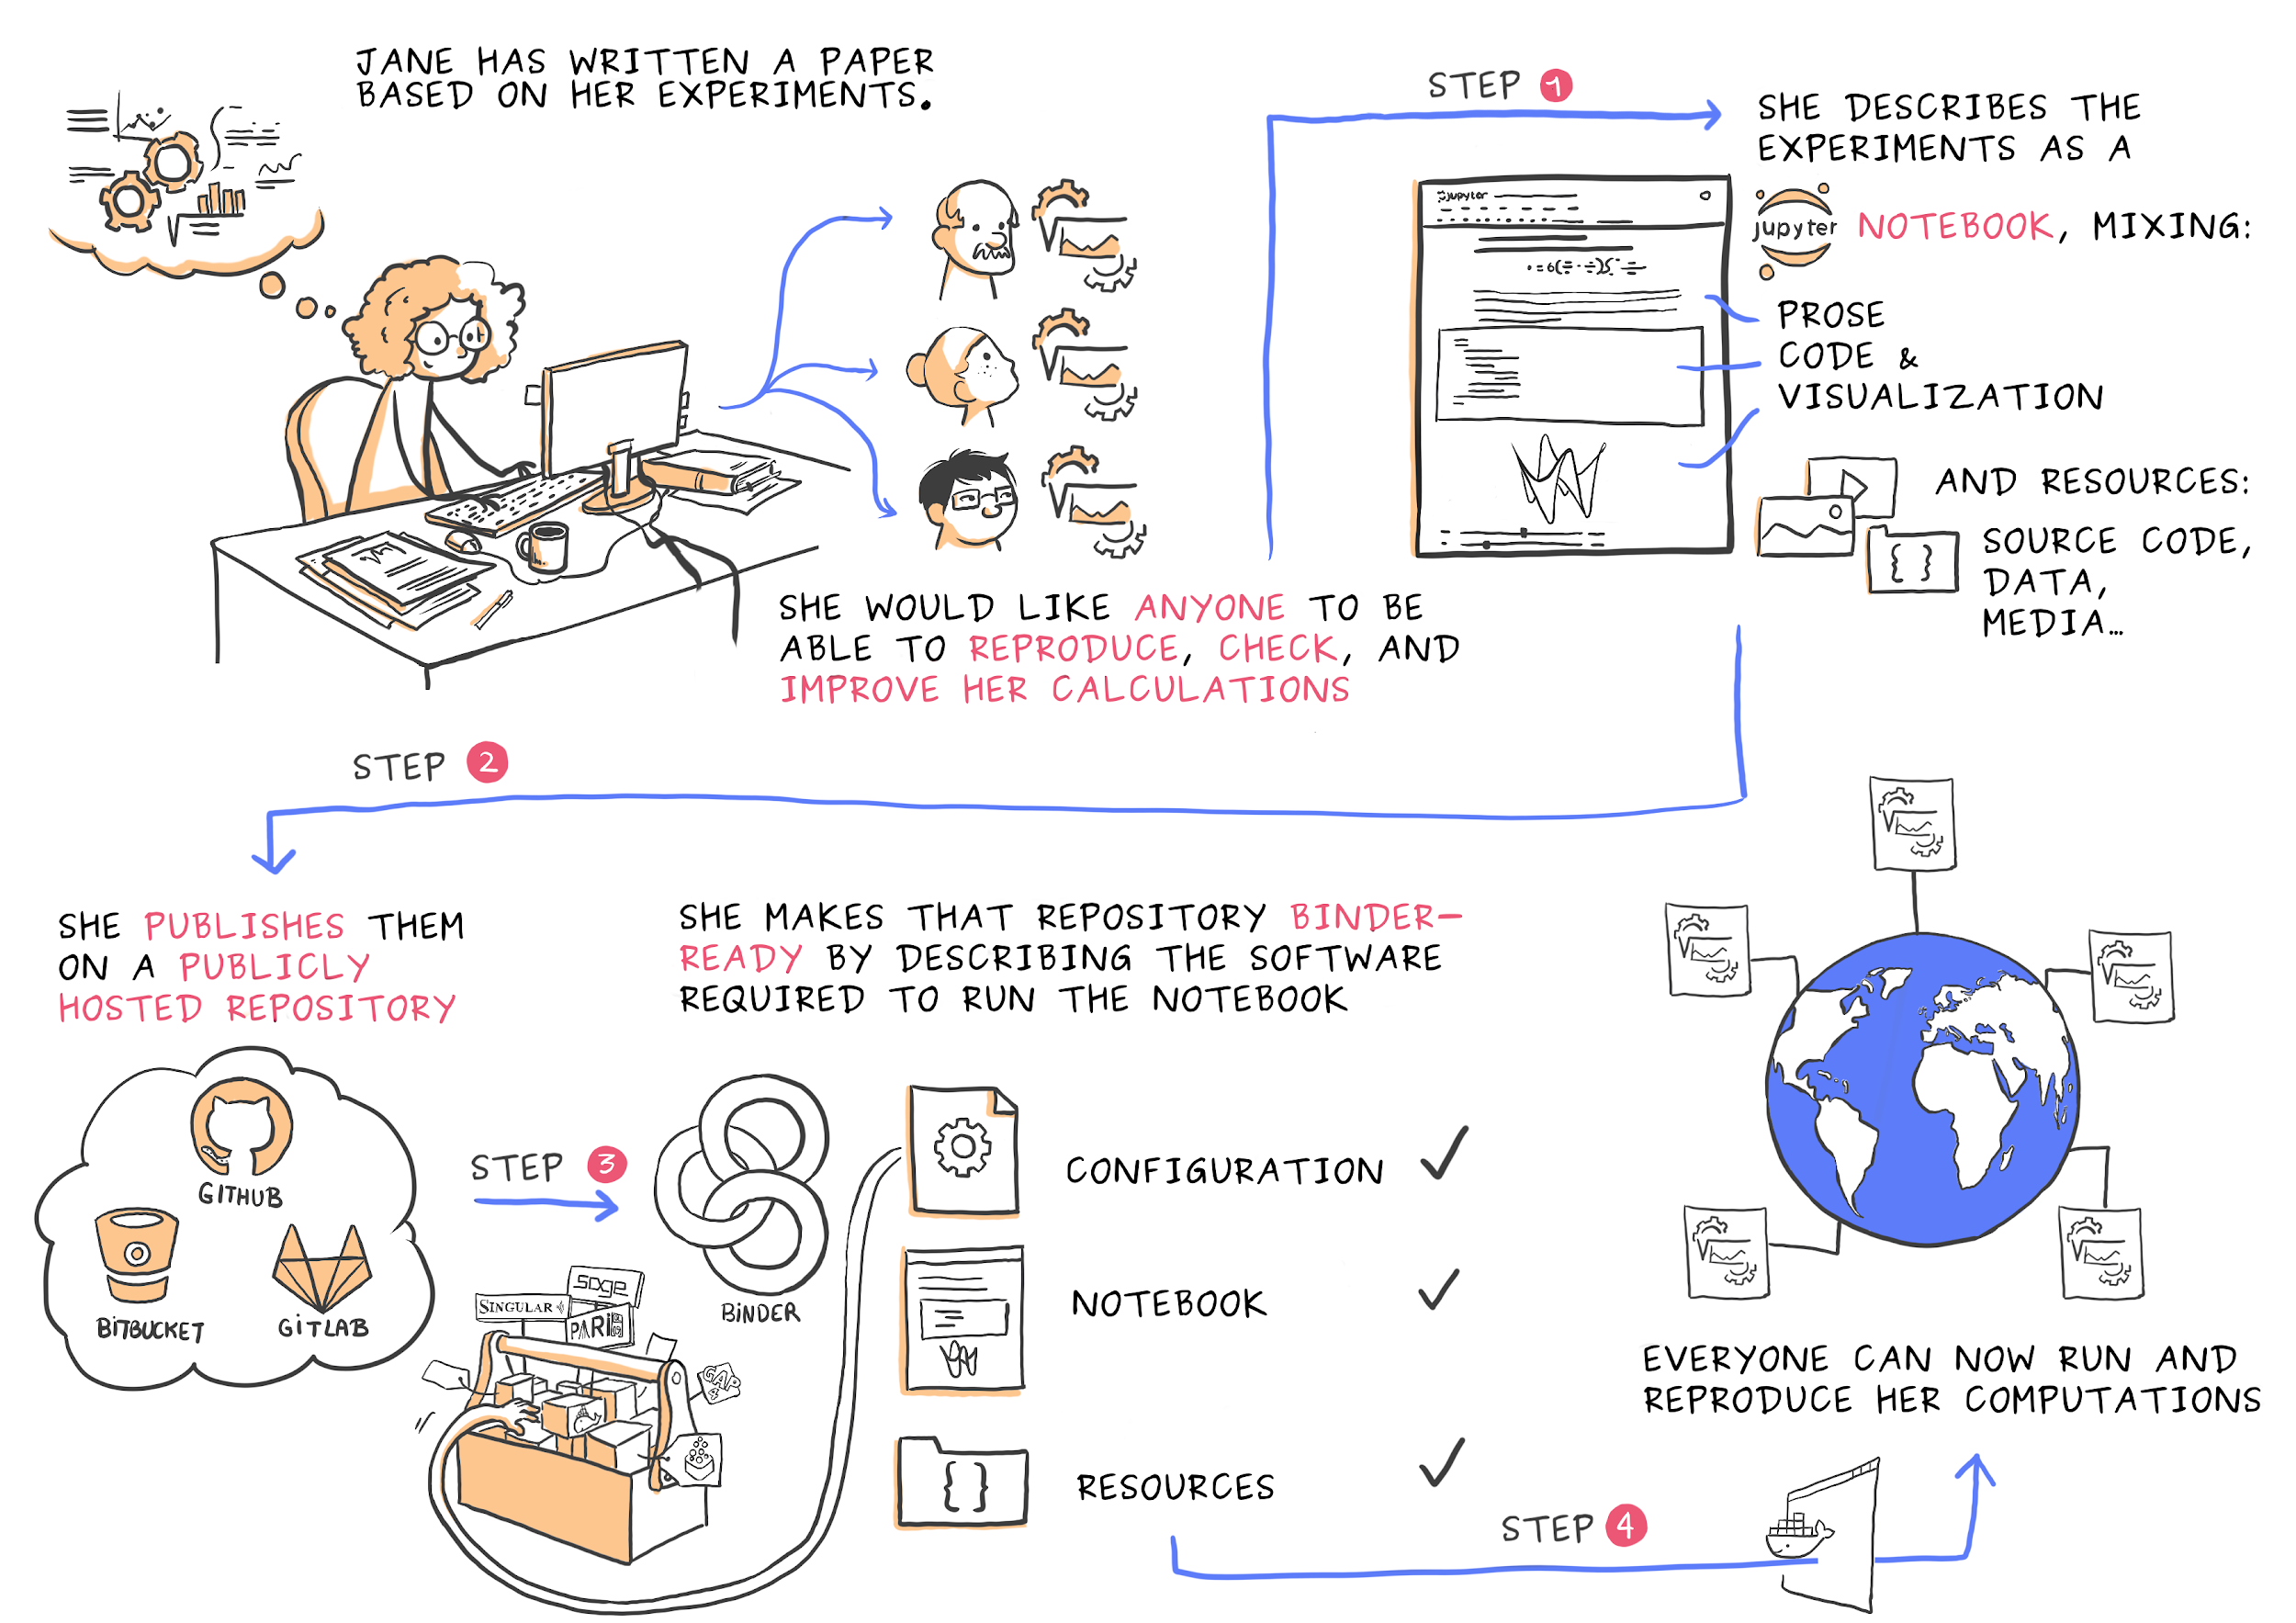
\includegraphics[scale=0.04]{imagenes/reproducibilidad.png}};
 \end{tikzpicture}
 
\end{center}
\end{frame}


\begin{frame}[fragile]
\frametitle{LA-CoNGA: Malla curricular}
\begin{center}
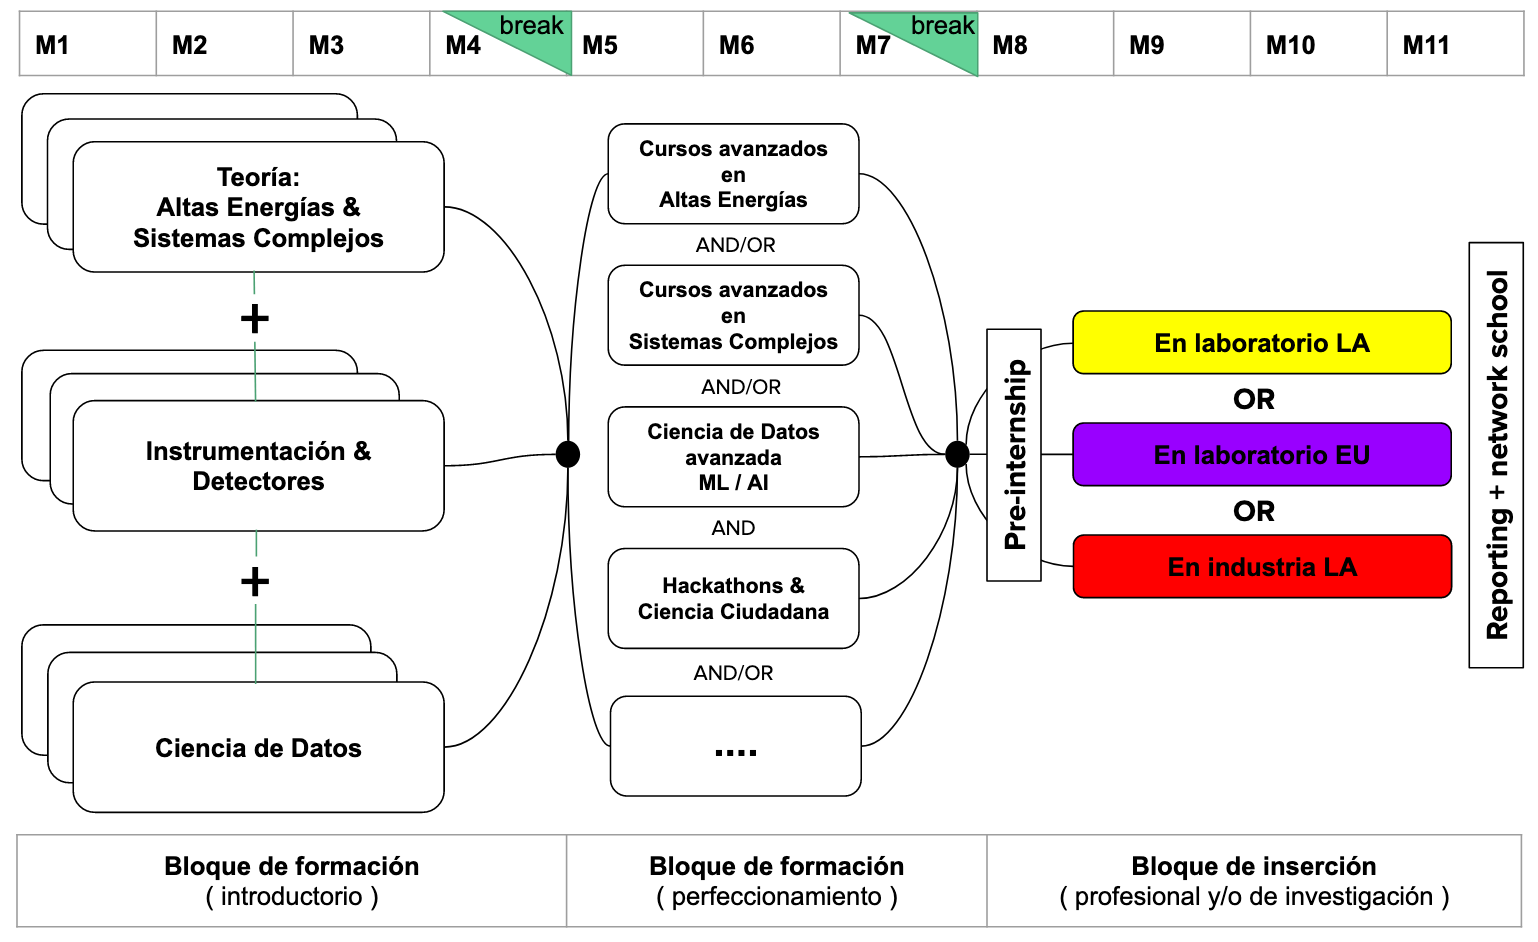
\includegraphics[scale=0.45]{imagenes/MetPlat.png}
\end{center}
\end{frame}

\note{sociosCienInd}





